\documentclass[../ECON-281-Notes.tex]{subfiles}
\begin{document}
\chapter{Consumer Preferences and Utility}
\begin{Definition}{Utility} 
  Satisfaction that you get from consuming a certain basket or bundle or combinations of goods.
\end{Definition}
There are multiple ways to measure utility: 
\begin{itemize}
  \item \textbf{Cardinal approach} Assume we can measure utility in \textbf{utiles}; a unit of measuring utility. We can measure this by using a table of values that contains $Q$, and $T_u$.
  \item \textbf{Ordinal approach} If we cannot measure utility but can rank the different bundles from the least to the most preferred. We can show these different ranks of utilities from an indifference curve.
\end{itemize}

\begin{Definition}
  {Preference}
  Indicates how a consumer rank different bundles.
  
  These preferences have certain properties:
  \begin{enumerate}
    \item They are complete AKA they must have an order function to rank these bundles, Note the ranking also includes indifference meaning both bundles are equally preferable.
    \item Transitive or logical ranking i.e., $A > B \text{ and } B > C \to A > C$.
    \item More is better than less, the goods that we study are economic goods not economic bads or regression.
  \end{enumerate}
\end{Definition}

\section{Indifference curve}
\begin{Definition}
  {Indifference Curve}
  Shows the different combinations (bundles) of any two goods that give the consumer the same level of utility.
  
  Along the same indifference curve, the level of utility is constant.

  The farther the curve is to the right and up the higher the overall amount of utility.

  We use the indifference curve to show ordinal utility of bundles.
\end{Definition}
\begin{figure}[!h]
  \centering
  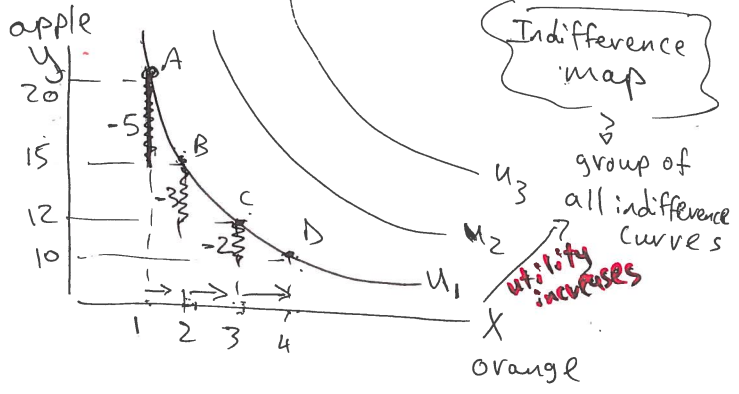
\includegraphics[width=0.8\columnwidth]{../assets/indifference_curve.png}
  \caption{Indifference Curve}
  \label{fig:assets-indifference_curve-png}
\end{figure}

Notice that the indifference curve is negatively slope. For consumers with a fixed level of utility there can only be trade-offs between one good or another. 
When the consumer make a single unit of trade-off between two goods it is called the \textbf{Marginal Rate of Substitution} or \textbf{MRS} which is the slope of the indifference curve at a given combinations of goods.

\begin{DndSidebar}[color=PhbLightGreen]{MRS Equations}
  \begin{equation}
    MRS_{xy} = \frac{-\Delta y}{\Delta x} = -\frac{M_{ux}}{M_{uy}}    
  \end{equation}
  or another way to understand is how much to give up $y$ to gain a single $x$. 
  \begin{equation}
    MRS_{yx} = \frac{-\Delta x}{\Delta y} = -\frac{M_{uy}}{M_{ux}}
  \end{equation}
  this is the inverse of the previous equation. How much to give up $x$ to gain a single $y$.
  \\~\\
  The best way to understand either form of $MRS$ is to look at the order of the subscripts. The first good is what you want to gain and the second is what you have to give up. 
\end{DndSidebar}


\begin{DndSidebar}[color=PhbLightGreen]{Law of diminishing MRS}
  The consumer is ready to give up less and less from one of the goods to get an extra unit from the other.
  That is why the difference curves are convex to the origin. 
\end{DndSidebar}

\begin{Note}
  Indifference curves cannot intersect between each other, if they do they violate the transitivity rule of preferences.
  Nor can they be thick because you can have a one combination of goods with a higher overall quantity but have the same utility as another combination of goods with a lower overall quantity. 
\end{Note}

\subsection{Cobb-Douglas Utility Function}
This is a utility function based on the following form
\begin{equation}
  u = Ax^{\alpha} y^{\beta}
\end{equation}
where $A$, $\alpha$, and $\beta$ are constant numbers

The Marginal Rate of Substitution using the Cobb-Douglas function is do
\begin{equation}
  MRS_{XY} = \frac{M_{ux}}{M_{uy}} = \frac{Y}{x}
\end{equation}
\begin{equation}
  MRS_{YX} = \frac{M_{uy}}{M_{ux}} = \frac{X}{Y}
\end{equation}


\section{Shape of different indifference curves}
There are many different shapes or classes of indifference curves
\subsection{Cobb-Douglas}
This is based on the convex to origin curve as shown in \cref{fig:assets-indifference_curve-png}. The MRS is diminishing.

\subsection{Perfect Complements}
The indifference curve is L-shaped the two goods must be used together in fixed proportion. 
The MRS is 0 as the consumer cannot substitute gone good for the other good.
\begin{equation}
  u = A\ \text{min}(ax, by)
\end{equation}
This function is called the Leoutief utility function where $a$ and $b$ are the proportions by which good $x$ and $y$ are used.

\subsection{Perfect Substitute}
Consumers consume any of the two goods or a combinations of both, the MRS constant throughout the entire indifference curve.
\begin{equation}
  U = ax + by
\end{equation}
This is called the linear utility function.

\subsection{Quasilinear Utility Function}
This utility function has a linear component for one good and a non-linear component for the other. The MRS is not constant.
Example:
\[ 
u = x + \ln y 
\] 

There are many functional forms for this utility function.



\end{document}
